\documentclass[]{article}
\usepackage{graphicx}
\graphicspath{ {./images/} }
\usepackage{caption}
\usepackage{subcaption}
\usepackage{amsthm}
\usepackage{amsfonts}
\usepackage{amsmath}
\usepackage{amssymb}
\usepackage{mathrsfs }
\newtheorem{mydef}{Definition}[section]
\newtheorem{mytheorem}{Theorem}[section]
\newcommand{\mathleft}{\@fleqntrue\@mathmargin0pt}

\title{Master Thesis -- Prove Problem}
\author{Kefang Ding} 
\date{\today}
\begin{document}
\maketitle
\hrulefill
\hrulefill 
\section{Introduction}
This article is used to explain the difficulty I confront about proving the soundness of generated model.
In the first phrase of algorithm, the existing model, positive event log and negative event log are used to generate a new directly-follows graph. Based on Inductiver Miner, this graph is transformed into a sound petri net without long-term dependency. 

In the next phase, our algorithm focuses on detecting and adding long-term dependency in Petri net. We define, if the supported connection on the set pair of xor branches is over a threshold, pair has significant correlation.Therefore, this pair has long-term dependency.

During the implementation, it comes clear that supported connection only on the positive and negative event log is not enough, since the existing model can keep some directly-follows relations about xor branches which do not show in the positive event log or shows only in negative event log. Consequently, when we detect this long-term dependency on those xor branches, there is no evidence of long-term dependency on those xor branches. It results in an unsound model as shown in Fig , since those xor branches can't get fired to consume the tokens generated from the choices before.
%% insert one unsound model here and point out the situations. 
\begin{figure}[!h]
	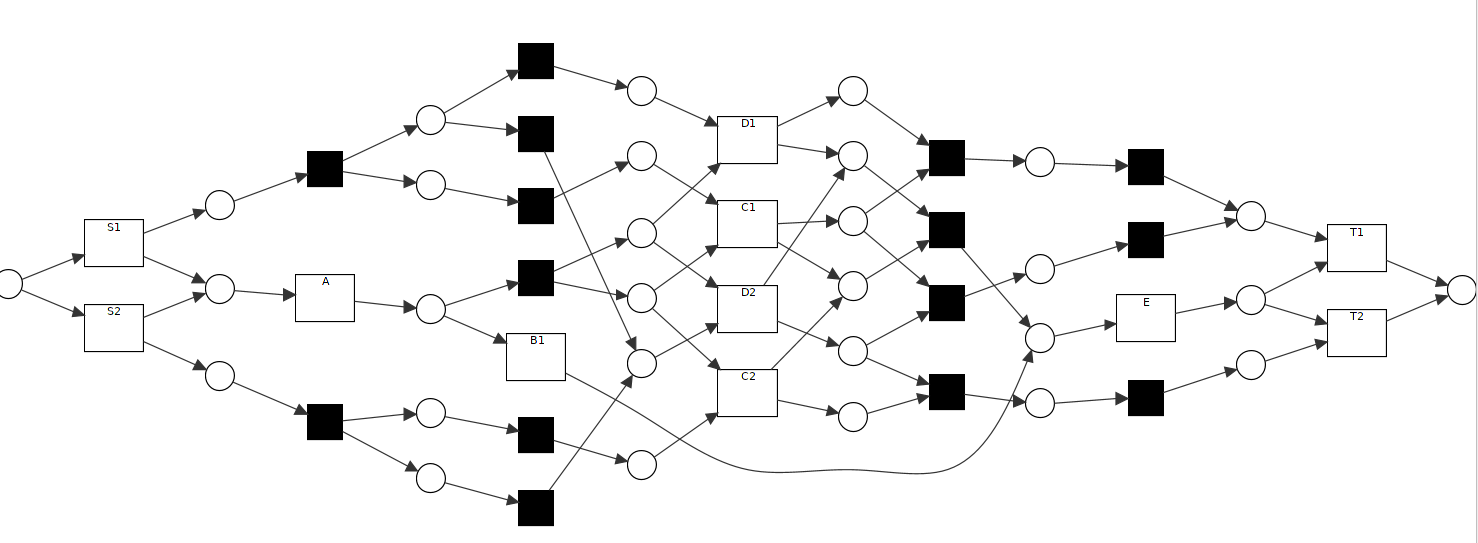
\includegraphics[width=\textwidth]{PN_tc_and_03_01.png}
	\caption{Unsound Repaired Model at Transition B1.}
	\label{fig:unsound_example}
\end{figure}
\section{Problem Description}
To make the generated Petri net sound, we propose a method to incorporate the existing model on the long-term dependency detection. The definition \ref{def: supported-connection} is rephrased into weight. 
\begin{mydef}[Rephrased Correlation of xor branch] The correlation for two branches is expressed into
	\[Wlt(XORB_X,XORB_Y)= Wlt{ext}(XORB_X, XORB_Y) + Wlt{pos}(XORB_X, XORB_Y) -Wlt{neg}(XORB_X, XORB_Y)\], where 
	$W_lt{ext}(XORB_X, XORB_Y)= \frac{1}{\#XORB_Y}$, $\#XORB_Y$ means the number of possible  directly-follows xor branches ${XORB_Y}$ after $XORB_X$. \\ \\
	$Wlt{pos}(XORB_X, XORB_Y)= \frac{F_{pos}(XORB_X, XORB_Y)}{F_{pos}(XORB_X, *)}$, \\
	$Wlt{neg}(XORB_X, XORB_Y)= \frac{F_{neg}(XORB_X, XORB_Y)}{F_{neg}(XORB_X, *)}$, \\	
\end{mydef}
The $F_{pos}(XORB_X, XORB_Y)$ and $F_{neg}(XORB_X, XORB_Y)$ are the frequency of the coexistence of $XORB_X$ and $XORB_Y$, respectively in positive and negative event log.

With this rephrased definition, to make the model sound, we need to prove, if there is a xor branch $XORB_Y$ in the generated process tree, there must exist one long-term dependency related to it, $\exists XORB_X, Wlt(XORB_X,XORB_Y) > lt-threshold$. We formalize this problem. Else, the model can't be sound!!
\begin{mytheorem}
	Given a process tree, a pair of xor branch set, $(B_A,B_B)$ with $B_A={XORB_{X1}, XORB_{X2},...XORB_{Xm}}, B_B={XORB_{Y1}, XORB_{Y2},...XORB_{Yn}}$, the obligatory part between $B_A$ and $B_B$ is marked M, it is to prove:: \\
	for one xor branch $XORB_Y$, if $W(M, XORB_Yj) > threshold$, \\ then there exists one $XORB_Xi$ with 
	\[Wlt(XORB_Xi, XORB_Yj)> lt_threshold\]. 
\end{mytheorem}
Given a simplified scenes, it is listed in Fig \ref{fig:simplified-graph-model}, if there exists directly-follows relation of M and Y1, then there must exist one long-term dependency of Xi and Y1. 

\begin{figure}[!h]
	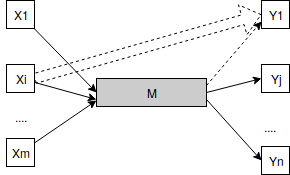
\includegraphics[width=\textwidth]{RelationOfThreshold-LTThreshold.png}
	\caption{Unsound Repaired Model at Transition B1.}
	\label{fig:simplified-graph-model}
\end{figure}

The definition of $W(M, XORB_Yj)$ is reviewed below.
\begin{mydef}[Assign new weights to graph $G_{new}$]
	there are three weights from $G_{pos}$, $G_{neg}$ and $G_{ext}$, the new weight is 
	\begin{itemize}
		\item For one directly-follows relation, \[ Weight(E_{G_{new}}(A,B)) = Weight(E_{G_{pos}}(A,B)) + Weight(E_{G_{ext}}(A,B)) - Weight(E_{G_{neg}}(A,B))\]
		\item Given a directly-follows graph G(L), the weight of each directly-follows relation is defined as \[ Weight(E(A,B)) = \frac{Cardinality(E(A,B))}{Cardinality(E(A,*))}  \] 
	\end{itemize}
\end{mydef}

When prove by contradiction, we assume that the opposite proposition is true. If it shows that such an assumption leads to a contradiction, then the original proposition is valid. 
\begin{mytheorem}
	for one xor branch $XORB_Y$, if $W(M, XORB_Yj) > threshold$, \\ there exists no one $XORB_Xi$ with 
	\[Wlt(XORB_Xi, XORB_Yj)<lt-threshold\]. 
\end{mytheorem}

Or we change to another thinking way to get the relation of threshold and lt-threshold, such that we have the theorem valid. Then we rephrase the question into
\begin{mytheorem}[Another way of thinking]
	Given a process tree, a pair of xor branch set, $(B_A,B_B)$ with $B_A={XORB_{X1}, XORB_{X2},...XORB_{Xm}}, B_B={XORB_{Y1}, XORB_{Y2},...XORB_{Yn}}$, the obligatory part between $B_A$ and $B_B$ is marked M. If,\\
	for one xor branch $XORB_Y$, if $W(M, XORB_Yj) > threshold$, \\ there exists one $XORB_Xi$ with 
	\[Wlt(XORB_Xi, XORB_Yj)> lt-threshold\]
	What is the relation of threshold and lt-threshold?? 
\end{mytheorem}
If we expand the theorem, we need to prove 
\begin{mytheorem}[Relation of threshold and lt-threshold]
	What is the relation of threshold and lt-threshold, to make the following proposition valid. If 
	\begin{equation*}
	 \begin{gathered}
		W(M, XORB_Yj)  > threshold \\
	Weight(E_{G_{new}}(M, XORB_{Yj})) = Weight(E_{G_{pos}}(M, XORB_{Yj})) \\
	+ Weight(E_{G_{ext}}(M, XORB_{Yj})) 
	- Weight(E_{G_{neg}}(M, XORB_{Yj}))  > threshold \\
	\frac{1}{|Y*|} + \frac{\sum_{Xi}{Cardinality(M,Yj|Xi)}} {\sum_{Xi}{Cardinality(M,Y*|Xi)}}  
	- \frac{\sum_{Xi}{Cardinality(M,Yj|Xi)\prime}} {\sum_{Xi}{Cardinality(M,Y*|Xi)\prime}} \\
	\text{Then, exist one Yj with}\\
	Wlt(Xi, Yj)> lt-threshold \\
	Wlt{ext}(Xi, Yj) + Wlt{pos}(Xi, Yj) -Wlt{neg}(Xi, Yj) > lt-threshold\\
	\frac{1}{|Y*|} + \frac{Cardinality(M,Yj|Xi)} {Cardinality(M,Y*|Xi)}  
	- \frac{Cardinality(M,Yj|Xi)\prime} {Cardinality(M,Y*|Xi)\prime} > lt-threshold  \\
	\text{Or \textbf{there is a contradiction when all Yj}}\\
	Wlt(Xi, Yj)< lt-threshold\\
	\sum_{Xi} Wlt(Xi, Yj) < |X*|lt-threshold \\
	\frac{|X*|}{|Y*|} + \sum_{Xi}\frac{Cardinality(M,Yj|Xi)} {Cardinality(M,Y*|Xi)}  
	- \sum_{Xi}\frac{Cardinality(M,Yj|Xi)\prime} {Cardinality(M,Y*|Xi)\prime} < |X*|lt-threshold  \\
	 \end{gathered}
	\end{equation*}	
$Cardinality(M,Yj|Xi)$ means the frequency of coexistence of M and Yj given Xi in the trace in positive, while $Cardinality(M,Yj|Xi)\prime$ represents the frequency in negative. $Cardinality(M,Y*|Xi)$ is the sum frequency of set ${Y1,..Yj,..Yn}$, it equals to \[Cardinality(M,Y*|Xi) = \sum_{Yi}Cardinality(M,Yj|Xi)\]
\end{mytheorem}
If we set them into zero, there is a lot of existing edges kept into the old method with no evidence in event log to support the connection. 
\end{document}	